\ChapterImagePrelim[cap:cronograma]{Cronograma}{./images/fondo.png}\label{cap:cronograma}
\mbox{}\\
\noindent

El cronograma presentado (véase figura~\ref{fig:cronograma}) establece la planificación estratégica del proyecto en seis fases 
distribuidas a lo largo de 24 semanas(6 meses). Durante el primer mes, se desarrolla la Fase 1:Análisis de \NPO, orientada a la 
identificación de necesidades, problemas y oportunidades de la arquitectura tecnologíca actual, sirviendo como base para la toma
de decisiones posteriores.

En el segundo mes, se da inicio a la Fase 2:Búsqueda sistemática, la cual se extiende a las primeras del tercer mes y tiene
como propósito identificar herramientas, metodologías, estándares y buenas prácticas aplicables al fortalecimiento de la seguridad
en la infraestructura de computación en la nube. Posteriormente en el tercer y cuarto mes, se ejecuta la Fase 3:Diseño de prototipo, 
enfocada en la definición de la arquitectura propuesta y la selección de los componentes de seguridad a implementar.

Durante el quinto mes y el sexto mes, se desarrolla la Fase 4:implementación de la arquitectura, etapa en la cual se integran los 
controles, herramientas y configuraciones de seguridad dentro de la infraestructura tecnologíca actual con el apoyo del %\UTM.
De manera complementaria, en el sexto mes se lleva a cabo la Fase 5:Validación de la arquitectura, orientada a verificar el correcto
funcionamiento de la propuesta implementadda y evaluar su alineación con los objetivos de seguridad establecidos.

Finalmente la Fase 6:Difusión y documentación se ejecuta de forma transversal desde etapas intermedias del proyecto hasta su cierre,
permitiendo el registro continuo de avances, resultados, decisiones técnicas y hallazgos relevantes. Este cronograma no solo facilita 
la organización temporal de actividades, sino que también constituye una herramienta clave para la gestión de recursos, el seguimiento 
del progreso y el cumplimiento de los objetivos del trabajo de grado.


\begin{figure}[H]
	\centering
	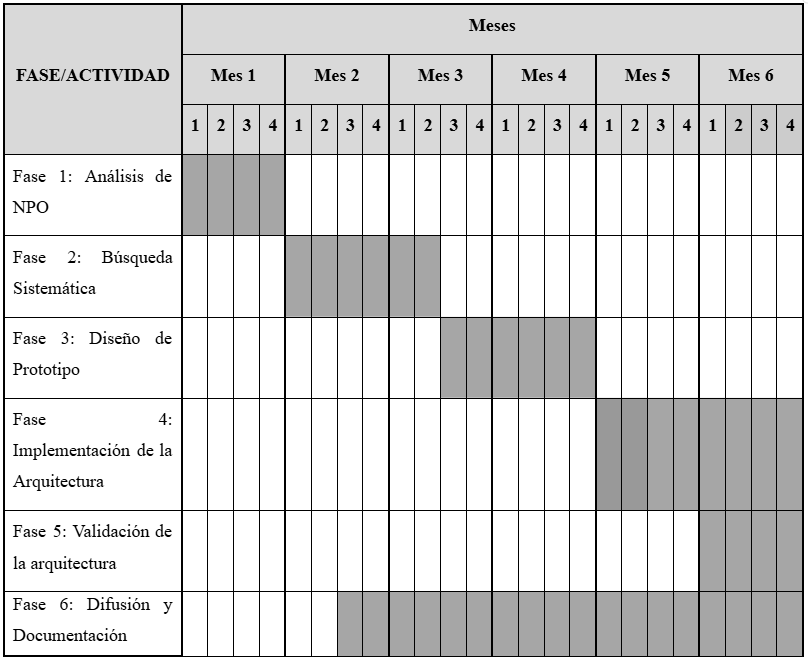
\includegraphics[scale=0.5]{tablas-images/partes/01-generalidades/cronograma.png}
	\caption{Cronograma de actividades del proyecto.}\label{fig:cronograma}
\end{figure}
